%%%%%%%%%%%%%%%%%%%%%%%%%%%%%%%%%%%%%%%%%
% University/School Laboratory Report
% LaTeX Template
% Version 3.1 (25/3/14)
%
% This template has been downloaded from:
% http://www.LaTeXTemplates.com
%
% Original author:
% Linux and Unix Users Group at Virginia Tech Wiki 
% (https://vtluug.org/wiki/Example_LaTeX_chem_lab_report)
%
% License:
% CC BY-NC-SA 3.0 (http://creativecommons.org/licenses/by-nc-sa/3.0/)
%
%%%%%%%%%%%%%%%%%%%%%%%%%%%%%%%%%%%%%%%%%

%----------------------------------------------------------------------------------------
%	PACKAGES AND DOCUMENT CONFIGURATIONS
%----------------------------------------------------------------------------------------

\documentclass[a4paper, 11pt]{article}

\usepackage{graphicx} % Required for the inclusion of images
\usepackage{natbib} % Required to change bibliography style to APA
\usepackage{amsmath} % Required for some math elements 
\usepackage[utf8]{inputenc} % polish characters
\usepackage[margin=1in]{geometry}
\usepackage[section]{placeins}
\usepackage{tabulary}
\usepackage{caption}
\usepackage{array}
\usepackage{color, colortbl}
\newcommand{\mc}[3]{\multicolumn{#1}{#2}{#3}}
\definecolor{Gray}{rgb}{.8,.8,.8}

%\setlength\parindent{0pt} % Removes all indentation from paragraphs

\renewcommand{\labelenumi}{\alph{enumi}.} % Make numbering in the enumerate environment by letter rather than number (e.g. section 6)

%\usepackage{times} % Uncomment to use the Times New Roman font

%----------------------------------------------------------------------------------------
%	DOCUMENT INFORMATION
%----------------------------------------------------------------------------------------

\title{Softcomputing \\ Neural network \\ Report} % Title

\author{Arkadiusz \textsc{Szydełko} 184626 \\ Tomasz \textsc{Kuchne} 184674} % Author name

\date{\today} % Date for the report

\begin{document}

\maketitle % Insert the title, author and date

% If you wish to include an abstract, uncomment the lines below
% \begin{abstract}
% Abstract text
% \end{abstract}

%----------------------------------------------------------------------------------------
%	SECTION 1
%----------------------------------------------------------------------------------------

\section{Presentation of the problem}
\label{problem_presentation}
The idea behind the project is to translate written by hand text to a machine text. There are a few problems to solve. The first one is to convert graphical image to number representation of each character. This part is already done, there are matrix representations of each character. The rest of the process has to be implemented.
 
The main problem of this project is to convert given matrices to real characters. Given matrices could not perfectly reflect correct representations of coded characters. There can be several problems, e.g. matrices can contain noises, values in different positions, values could be different or the matrices can even be different sizes.

Figures \ref{nodes_changed}, \ref{noises} and \ref{values_sizes_changed} shows more precariously how the data is represented and what are the possible problems.

\begin{figure}[h]
\begin{center}
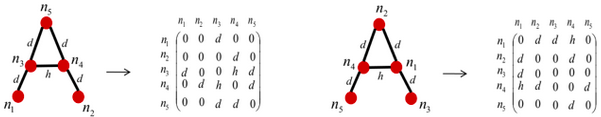
\includegraphics[width=0.85\textwidth]{images/nodes}
\caption{Different position of nodes.}
\label{nodes_changed}
\end{center}
\end{figure}

On the figure \ref{nodes_changed}, it can be observed that, when convention of node numeration will change, the matrix will be different, even if it contains the same number of values of each type. 

Each letter has different number of nodes. The nodes are representing a critical points of the letter. E.g. letter A has 5 nodes, which connected in a correct way construct letter A. The values itself are representing connection type between letter's nodes. Overall there are 4 correct type of connections, but it happens that matrices will contain other not specified types caused by errors. Including incorrect types the number of types which appear in the data is 8.

Figures \ref{noises} and \ref{values_sizes_changed} represents other types of errors in matrices, with noise, different values and different matrix size.

\begin{figure}[ht]
\begin{center}
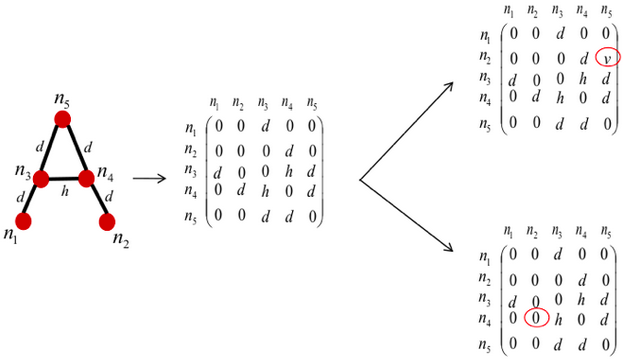
\includegraphics[width=0.85\textwidth]{images/noise}
\caption{Noise example.}
\label{noises}
\end{center}
\end{figure}

\begin{figure}[ht]
\begin{center}
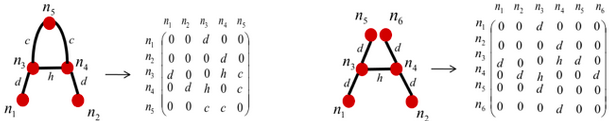
\includegraphics[width=0.85\textwidth]{images/values}
\caption{Different values and sizes.}
\label{values_sizes_changed}
\end{center}
\end{figure}
 
%----------------------------------------------------------------------------------------
%	SECTION 2
%----------------------------------------------------------------------------------------

\section{Data preparation}

The data to work on is provided in a text files where each line represent different letter and can be transformed into matrix. Data which represent alphabet is shown in Figure \ref{alphabet}. The first number in the line determinate how many columns given matrix contain, rest of numbers in the line are values of matrices.

Each letter is a matrix of different size and is not in a binary representation, which is not suitable for neural network usage. Because of that the data need to be transformed into alternative representation.

The biggest matrix which appear in the test cases has size \(10x10\), based on this assumption all other matrices were resized to fit this size. Matrices were resized by adding 0 on the right and bottom sides. After that values needed to be transformed into binary representation. To accomplish that each position was extended (in width of the matrix) to have 4 digits. As mentioned in section \ref{problem_presentation}, the highest value that appear in test cases is 8 and to represent 8 in binary code, 4 positions are needed.

After all transformations all matrices has the same size, contains only binary values and their size is \(40x10\). Which is a result of calculations \ref{bin_representation_size}. E.g. representation of the letter A is illustrated in figure \ref{coded_letter}.

\begin{equation}
(\mathrm{10\;columns} * \mathrm{4\;bit})\;x\;\mathrm{10\;rows} = \mathrm{40\;columns\;x\;10\;rows}
\label{bin_representation_size}
\end{equation}

\begin{figure}[ht]
\begin{center}
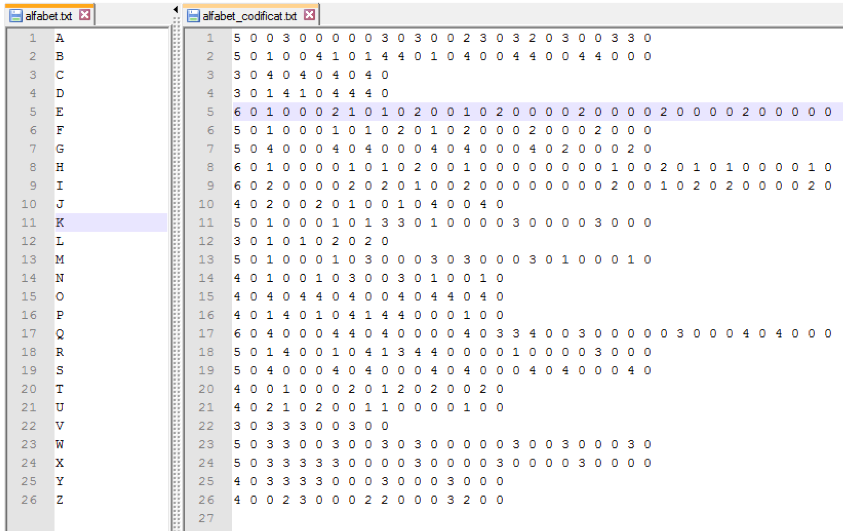
\includegraphics[width=0.85\textwidth]{images/alphabet}
\caption{Alphabet representation.}
\label{alphabet}
\end{center}
\end{figure}

\begin{figure}[ht]
\begin{center}
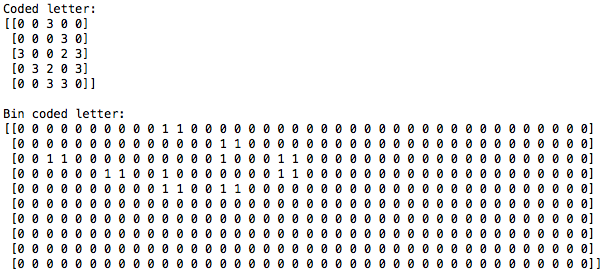
\includegraphics[width=0.85\textwidth]{images/coded_letter}
\caption{Representation of coded letter A.}
\label{coded_letter}
\end{center}
\end{figure}

%----------------------------------------------------------------------------------------
%	SECTION 3
%----------------------------------------------------------------------------------------

\section{Neural network}

Network used in the project is a multilayer perceptron network with recurrent connections in the hidden layer. It is characteristic of having multiple layers of nodes. Two obligatory layers, input and output layers and hidden layers (one or more). The recurrent part in addition to a traditional connections in multilayer perceptron, has also connections between each node in the hidden layer, including node connections to themselves. This approach is useful to handle sequential data. Because it can use their internal memory to process sequences it is an ideal solution for handwriting recognition. Unfortunately the data provided to this project is not suitable to fully make use of this kind of network, but it was discussed on project meeting to stay with that solution.

\subsection{Structure}

The network created for the project has 400 nodes in input layer, one hidden layer where various number of nodes were tested and 26 nodes in output layer. 
The size of input layer is caused by sizes of data matrices, which are of size \(40x10\). After translating that matrix into a vector, which is required as an input structure, it will be with a length of 400.
The size of hidden layer was tested for various numbers of nodes, but the best results were achieved with 200 nodes in the hidden layer. 
The size of output layer is equal to 26, because the alphabet contains 26 letter and implementation of network in used library is working in a way that the output has only one value, which is equal to 1, the rest are 0.

Total number of connections in the network is equal to 125 200. With the assumption that there are 200 nodes in hidden layer. The value was calculated by equation \ref{number_of_connections}.

\begin{equation}
N_{w}\;=\;N_{il} * N_{hl} + N_{hl} *N_{hl} + N_{hl} * N_{ol}
\label{number_of_connections}
\end{equation}

\begin{tabular}{@{}>{$}l<{$}l@{}}
N_{w} & - Number of connections\\
N_{il} & - Number of nodes in input layer\\
N_{hl} & - Number of nodes in hidden layer\\
N_{ol} & - Number of nodes in output layer\\
\end{tabular}

\subsection{Training}

The network was trained with backpropagation method. Number of training episodes was chosen based on total error value. Each time learning was started, total error value at the beginning was decreasing to some point and then when the training was continued, the value was slowly growing with each next episode. The final number of training iteration was chosen on a point where total error value was the smallest possible, which was different for various network configurations.

%----------------------------------------------------------------------------------------
%	SECTION 4
%----------------------------------------------------------------------------------------

\section{Tests}

There is a set of six tests cases. Each of them contains different types of errors.

\begin{tabular}{p{0.3cm}p{14cm}}
\\
\(T_{1}\) & - Test case does not contain any errors.\\
\(T_{2}\) & - Test case contains mixed rows and columns.\\
\(T_{3}\) & - Test case contains mixed rows and columns.\\
\(T_{4}\) & - Test case contains noise in matrices.\\
\(T_{5}\) & - Test case contains noise in matrices and changed values in correct positions.\\
\(T_{6}\) & - Test case contains noise in matrices, mixed rows and columns, changed values and changed matrix sizes.\\
\\
\end{tabular}

The most interesting results are presented in the table \ref{recognition}, for others configuration parameters the results ware not satisfactory. Following range of parameters were tasted:

\begin{tabular}{ll}
\\
Learning rate & - Values: 0,05 , 0,1 and 0,2.\\
Momentum & - Values: 0,1 and 0,2.\\
Nodes in hidden layer & - Values: 50, 100 and 200.\\
\\
\end{tabular}

\begin{center}
  \begin{tabulary}{\textwidth}{|C|C|C|C|C|m{0.8cm}|m{0.8cm}|m{0.8cm}|m{0.8cm}|m{0.8cm}|m{0.8cm}|}
  \hline
    No & Learning Rate & Momentum & Nodes in hidden layer & Training iterations & \(T_{1}\) & \(T_{2}\) & \(T_{3}\) & \(T_{4}\) & \(T_{5}\) & \(T_{6}\) \\
    \hline
    1 & 0,05 & 0,1 & 50 & 200 & 94\% & 68\% & 46\% & 96\% & 42\% & 88\% \\
    \hline
    2 & 0,05 & 0,1 & 200 & 180 & 97\% & 65\% & 53\% & 98\% & 43\% & 88\% \\
    \hline
    3 & 0,05 & 0,2 & 50 & 100 & 100\% & 72\% & 51\% & 100\% & 47\% & 91\% \\
    \hline
    \rowcolor{Gray}
    4 & 0,05 & 0,2 & 200 & 120 & 100\% & 70\% & 61\% & 99\% & 48\% & 91\% \\
    \hline
    5 & 0,1 & 0,1 & 50 & 40 & 97\% & 68\% & 46\% & 97\% & 43\% & 88\% \\
    \hline
    6 & 0,1 & 0,2 & 100 & 40 & 100\% & 70\% & 57\% & 100\% & 46\% & 91\% \\
    \hline
  \end{tabulary}
  \captionof{table}{Recognition results.}
  \label{recognition}
\end{center}

From performed tests overall the best configuration is the number 4 from the table \ref{recognition}. It achieved the highest percentage of correct recognition in most test cases.

The results shows in what situations the network is doing well or not. Clearly the easiest case for the network is to recognize letters with noise, the results for this test case were almost 100\% across different configurations.

The network has problems when letters are represented correctly, but in different order of nodes, test cases no. 2 and 3. The results vary from 46\% to 72\% of correct recognition. But it is understandable when taking into assumption the way that neural network works and the way of data binary representation. After such a changes matrix can clearly start to look similar to different letter.

The worst cases for the network to deal with are noises connected with changed values, illustrated in figure 2 and 3. The reason is probably similar to problems with test cases no. 2 and 3, but results are much worst. In any configuration even 50\% of correct recognition was not achieved.

The last test case which contains all kind of errors went well with average of 90\% of correct recognition. Wrong recognition was mostly connected with errors of different order of nodes and changed values.

%----------------------------------------------------------------------------------------
%	SECTION 5
%----------------------------------------------------------------------------------------

\section{Implementation}

Project was implemented in Python 2.7, with additional libraries to handle network structure and learning algorithms. Following libraries were used:

\begin{itemize}
  \item PyBrain - library which provide tool to manage different types of machine learning procedures and structures. It contains modules to handle neural networks.
  \item NumPy - package for scientific computing with Python, with native functions written in C/C++ for faster computations and more efficient number date representations. It also provide functions for various matrices operations.
  \item SciPy - module to support mathematics operation in Python.
\end{itemize}

Project was implemented in a way for easy possibility to change different network parameters in order to test various learning and network options. Project also contain analytics module which create a special files with analysis of each computed letter. The analysis contains given letter, expected letter and obtained letter in all possible representations (as letter, as bin matrix and as original matrix) to easily investigate network behaviors.

%----------------------------------------------------------------------------------------
%	SECTION 6
%----------------------------------------------------------------------------------------

\section{Conclusions}
With right tools basic neural networks can be easily implemented. Neural networks are great for problems connected with data that contains noise or are deformed. Unfortunately it is not good solution for modified data sets, where some values are different then they should be (problems illustrated in figure \ref{values_sizes_changed}).


%----------------------------------------------------------------------------------------
%	BIBLIOGRAPHY
%----------------------------------------------------------------------------------------

%\bibliographystyle{apalike}

%\bibliography{sample}

%----------------------------------------------------------------------------------------


\end{document}